\documentclass[final]{report}
% Includes
% *** GRAPHICS RELATED PACKAGES ***
%
\usepackage[pdftex]{graphicx}
\graphicspath{}
\DeclareGraphicsExtensions{.pdf,.jpeg,.png}
\usepackage{listings}
\usepackage{amsmath}
\usepackage{amssymb} % more math symbols
\usepackage{esint} % more math symbols
\usepackage{fullpage}
\usepackage[hidelinks]{hyperref} % doesn't work if draft mode on
%% Add bibliography to the table of contents and remove entries for lists of tables/figures
\usepackage[nottoc, notlot, notlof]{tocbibind}
%% Set vertical space between paragraphs and paragraph indent
%% (need to use 2019 version of texlive for these options to be available!)
\usepackage[skip=\baselineskip, indent=1.5em]{parskip}
%% Add "draft" watermark to each page
\usepackage{draftwatermark}
\SetWatermarkScale{5}

% Custom commands
%% Change titles of lists of Figures and Tables to custom ones
\renewcommand{\listfigurename}{Figures}
\renewcommand{\listtablename}{Tables}
%% Change default bibliography label to "References"
%\renewcommand\bibname{References}

\begin{document}

  \title{Brief Summary and Tutorial of the FEM Plasma Code: Zapdos}
  \date{October 2019}
  \author{Corey DeChant}
  \maketitle

  \chapter*{Summary}
    \addcontentsline{toc}{chapter}{Summary}
    \phantomsection
    The purpose of this tutorial document is to give the reader an overview of Zapdos and its capabilities. Within this tutorial document, there is a review of the finite element method (FEM) technique of transforming the strong form of an equation into its weak form. With this technique, we obtain the weak form of the multi-fluid approach to plasma modeling and the available physics within Zapdos. This document also reviews the object-oriented approach of MOOSE/Zapdos, the function of each object block, and the structure of these object blocks within an input file. There is a quick overview of MOOSE's GUI, Peacock, which is helpful for first time users of MOOSE and those with little/no experience with C++. With this knowledge, the tutorial document ends with a few examples of input files and a description of the plasma discharges that they incorporate.

  \chapter*{Acknowledgements}
    \addcontentsline{toc}{chapter}{Acknowledgements}
    \phantomsection
    We would like to acknowledge the following as collaborators with the support and development of Zapdos:
    \begin{itemize}
        \item University of Illinois at Urbana-Champaign: Laboratory of Computational Plasma Physics
        \item University of Notre Dame: Go Research Group
        \item University of California, Berkeley: Graves Lab
        \item Oak Ridge National Laboratory: Fusion Energy Division
    \end{itemize}
    We would also like to acknowledge the following as funding sources:
    \begin{itemize}
        \item United States Department of Energy through the Office of Science Graduate Student Research (SCGSR) Program
        \item National Science Foundation through the SI2-SSE Award \#1740300
        \item Idaho National Laboratory through the INL Graduate Fellowship Program
    \end{itemize}

  \tableofcontents

  \chapter{Introduction} \label{introduction}
  Zapdos is an open source plasma fluid code originally developed by Dr. Alexander Lindsay at North Carolina State University (NCSU). It is built as an application in the MOOSE (Multiphysics Object Oriented Simulation Environment) framework. The MOOSE framework is an object-oriented C++ finite element method (FEM) framework developed at Idaho National Laboratory for the purpose of solving highly coupled multiphysics problems. The MOOSE framework has several applications that are dedicated to particular areas of physics and that can be easily coupled together, Zapdos being the application for plasma simulation. \\
  \\
  Zapdos uses the multi-fluid approach (i.e. that each particle is treated with its own continuity equation). The electric field is treated with the electrostatic approximation and currently there is no magnetic field treatment in Zapdos. It is worth noting that there is currently an electromagnetic solver in development by NCSU's Casey Icenhour that can be coupled to Zapdos in the future. The plasma chemistry within Zapdos is treated by MOOSE's general chemistry application, CRANE. CRANE was developed by Shane Keniley at University of Illinois at Urbana-Champaign. The inner working of CRANE will not be discussed in this document, but the process of using CRANE within Zapdos will be discussed. For a more in-depth overview of CRANE, please visit \url{https://github.com/lcpp-org/crane}.\\
  \\
  The installation instructions for Zapdos can be found at \url{https://shannon-lab.github.io/zapdos/getting_started/}. By using these instructions, CRANE will be downloaded as a submodule of Zapdos. CRANE is then built as a library whose objects are accessible within Zapdos, enabling direct coupling of the two codes.

  \chapter{Brief Introduction to FEM and MOOSE Objects} \label{chapter2}
  \section{FEM: Strong to Weak Form}
  The complete process of the FEM will not be discussed in this tutorial document, but the main concept of transforming the strong form of an equation to the weak form will be reviewed. The equations in MOOSE/Zapdos are coded in the weak form, so understanding this concept is useful when adding physics to Zapdos. The strong form refers to the differential form of an equation. For an example, lets look at the classic diffusion problem of:

  \begin{equation}
      \nabla\cdot -D\nabla u = s(\mathbf{r})
  \end{equation}
  \\
  Where $D$ is the diffusion coefficient, $u$ is the species of diffusion, and $s(\mathbf{r})$ is the source term. Equation 2.1 would be classified as the strong form of the diffusion problem. To convert this into the weak form for FEM, one must multiply the equation by a test function $\psi_{i}$ and integrate over the whole domain of interest. All the terms will also be moved over to the left-hand side (LHS), resulting in the following:

  \begin{equation}
      \int_{\Omega}\psi_{i}\nabla\cdot -D\nabla u dV - \int_{\Omega} s(x) dV = 0
  \end{equation}
  \\
  Where $\Omega$ is the extent of the domain. Now the first term can be treated by using integration by parts, which gives:

    \begin{equation}
      \int_{\Omega}\nabla\psi_{i}\cdot D\nabla u dV - \int_{\partial\Omega}\psi_{i}D\nabla u\cdot \mathbf{n} dS - \int_{\Omega} s(x) dV = 0
  \end{equation}
  \\
  where $\partial\Omega$ is the domain boundaries and $\mathbf{n}$ is the normal vector to the boundary. Equation 2.3 contains the ``kernels" (e.g. the first and third term) and boundary conditions (e.g. the second term) that are entered into MOOSE/Zapdos. The rest of the FEM involves the discretization of the equation. For the purpose of this tutorial document, that process will be overlooked, but the fine details of the discretization process can be found in the third chapter of \cite{Alex_thesis}. In the example problems in this tutorial, the continuous Galerkin finite element method is utilized with linear Lagrange test functions. Solution of the resulting system of equations is obtained via Newton's Method.
  \section{MOOSE/Zadpos Objects}
  The rest of this chapter will consist of summaries for MOOSE/Zapdos object blocks. The object blocks are how input files are broken up into different significant parameters. These blocks can fall into one of the following categories: GlobalParams, Mesh, MeshModifiers, Problem, Variables, Kernels, AuxVariables, AuxKernels, Interfacekernels, BCs, ICs, Functions, Materials, Postprocessors, Preconditioning, Executioner, TimeStepper, and Outputs.
  \subsection{GlobalParams}
  The GlobalParams block is for defining parameters that appear in multiple blocks in a given input file. This is useful in particular for Zapdos, since Zapdos has scaling options for voltage and distance to better help with the conditioning of problems (e.g. sometimes it is computationally easier to define voltage in kV instead of V).
  \subsection{Mesh and MeshModifiers}
  The Mesh block is for creating a mesh or reading existing mesh files. MOOSE has its own mesh building feature -- more information can be found here: \url{https://mooseframework.org/source/mesh/GeneratedMesh}. MOOSE/Zapdos can also read a variety of mesh files. For the examples in this tutorial document, the meshes are created using the finite-element mesh generator, Gmsh \cite{Gmsh}. Naming of boundaries and domains can be defined in the mesh file itself, or in the MeshModifiers block. As the name suggest, the MeshModifier block modifies the mesh defined in the Mesh block. Such modifications can include stretching low dimension meshes into higher dimension and defining boundaries. For the following 1D example, a MeshModifier is used to defined to end points of the 1D mesh as boundaries.
  \subsection{Problem}
  The Problem block is where the type of problem to be solved is defined. By default, this is set to be FEProblem (containing one Nonlinear System to be solved), but other options (such as that for Eigenvalue problems) are available. Also, the coordinate system of the problems can be set in the Problem block. For the 2D example, an axial symmetric cylindrical system is used.
  \subsection{Variables and Kernels}
  The Variables block is where the variables of the problem are defined. As mentioned in Section 2.1, the default setting is a linear Lagrange basis function. The selection of these functions can highly depend on the types of problems and are beyond the scope of this tutorial. The Kernels block contains the physics of the problems, and in particular, the Kernel block contains the volume integrals found in the weak form of the set of equations (e.g. the first and third term of Equation 2.3).
  \subsection{AuxVariables and AuxKernels}
  The AuxVariables and AuxKernels blocks are similar to the Variables and Kernels blocks, but they contain for variables and terms not essential for solving the problem, but that still provide useful information. For an example, the electron density and potential would be considered variables, since they are essential for solving the multi-fluid method of plasma. The value of the electron current would be considered an AuxVariable (or auxiliary variable), since the current can be defined in terms of the electron density and potential.
  \subsection{InterfaceKernels}
  The InterfaceKernels block contains constraints or relationships between variables at the boundary of two domains. In order to use InterfaceKernels, interface boundaries must be defined to set the location of the constraint or relationship. In Zapdos, InterfaceKernels are used for equating the electron flux at the plasma-liquid interface.
  \subsection{BCs}
  The BCs block is for defining the boundary conditions of the problem. In FEM, there are two main types of boundary conditions, Dirichlet and Integrated BCs. The Dirichlet BC is an "NodalBC" in MOOSE (which is not integrated over the boundary) and directly defines the value of the variable at the boundary. For Zapdos, Dirichlet BCs are used to set the potential at boundaries to a sin function for RF discharges or zero for grounded walls. Integrated BCs are integrated over the boundary and are used for flux BCs in Zapdos.
  \subsection{ICs}
  The ICs block defines the initial conditions of the variables of the problem. Variables initial states can be setup as a uniform constant throughout the mesh, or be defined as a function of position.
  \subsection{Functions}
  The Functions block defines any functions that are used in the other blocks. Functions can be defined by position and time. Custom, parsed functions (via the ParsedFunction object) also allows for direct usage of common functions, such as trigonometric and logarithmic functions.
  \subsection{Materials}
  The Material block is used to define material properties within the mesh. In Zapdos, these properties include mass, mobility, diffusion coefficients for charged and neutral species, common physical constants, and reaction rates. It is worth noting that the reaction rates and electron mobility/diffusion coefficients are tabulated in a table provided by the user in terms of mean electron energy (usually solved from a Boltzmann solver). All rates and electron mobility/diffusion coefficients used in the tutorial examples comes form the work done by Lymberopoulos in \cite{1D_GEC} or by BOLSIG+.
  \subsection{Postprocessors}
  The Postprocessors block defines a variety of postprocessing operations. In the following examples, the post-processor of InversePlasmaFreq is used to find the inverse of the peak plasma frequency to help define the time steps.
  \subsection{Preconditioning}
  The Preconditioning block is to define any preconditioning processes needed to solve the problems. The following examples in this tutorial uses SMP (Single Matrix Preconditioner), which builds one preconditioning matrix based on the Jacobians in the Kernels. This setting requires more advanced understanding of solving nonlinear systems of equations and is beyond the scope of this tutorial.
  \subsection{Executioner}
  The Executioner block defines whether the problem to be solved is transient or steady-state, as well as various solver settings. For the problems in Zapdos, this setting is usually set to transient. For a transient problem, the end time, max time step and min time step can be defined in this block. For more advanced users, convergence tolerance and PETSc solver options are also defined in the Executioner block.
  \subsection{TimeStepper}
  The TimeStepper block determines the definition of the time steps. The two main time steppers used in Zapdos are IterationAdaptiveDT and PostprocessorDT. IterationAdaptiveDT will increase or decrease the time step depending of the convergence rate of the problem. PostprocessorDT uses a post-processor output to determine the time step (e.g. PostprocessorDT with the InversePlasmaFreq post-processor defines the time step as the inverse of the peak plasma frequency.
  \subsection{Outputs}
  The Output block defines the type of file used for the output file. The default output file type is an exodus file, which can the read with visualization application (such as ParaView). The name of the output file can also be defined in this block.
  \subsection{Actions}
  Actions are specialty blocks that are designed to construct other MOOSE objects. Two such Action blocks used in Zapdos and CRANE are the "DriftDiffusionAction" and "Reactions". Those two Actions let the user easily input the necessary kernels for the drift-diffusion/Electrostatic equations, and the necessary kernels and materials for the chemical reactions (respectively). More details about how to use Actions are in Section 4.1.
  \subsection{MultiApps and Transfers}
  The Multiapps block allows users to perform sub-simulations during the main simulation's run. The Transfers block, as the name suggests, is used to transfer values between main and sub-apps. Within Zapdos, MultiApps are needed to preform acceleration techniques, or to run coarser meshes for metastable densities alongside with finer mesh for electrons and ions.

  \chapter{Physics of Zapdos} \label{chapter3}
  \section{Weak Form of Multi-Fluid Plasmas}
  The physics of Zapdos are based on the multi-fluid approach to plasma simulation. With this approach, each particle is simulated with its own continuity equation in the form of:
  \begin{equation}
      \frac{\partial n_{j}}{\partial t}+\nabla\cdot\mathbf{\Gamma_{j}}=\sum{\mathbf{S_{iz}}}
  \end{equation}
  \\
  Where $n$ is the density, $j$ is the subscript for either electrons ($e$), ions ($i$) or metastables ($*$), $\mathbf{\Gamma}$ is the flux of the species, and $\mathbf{S_{iz}}$ is the source terms. The source terms are treated by CRANE and for the purpose of this tutorial, CRANE can handle one, two and three body reaction rates. It should be noted that Zapdos and CRANE can also treat the source terms in the form of Townsend coefficients. Since the tutorial example problems use reaction rates, that is the form discussed in this document. The form of these sources terms are:

  \begin{equation}
    \begin{gathered}
    \text{One Body:} \\
    \mathbf{S_{iz}}=vkn_{1} \\
    \text{Two Body:} \\
    \mathbf{S_{iz}}=vkn_{1}n_{2} \\
    \text{Three Body:} \\
    \mathbf{S_{iz}}=vkn_{1}n_{2}n_{3}
    \end{gathered}
  \end{equation}
  \\
  Where $v$ is the stoichiometric coefficient and $k$ is the rate coefficient. The flux of the particles are in the form of:

  \begin{equation}
      \mathbf{\Gamma_{j}}=\mu_{j}\mathbf{E}n_{j}-D_{j}\nabla n_{j}
  \end{equation}
  \\
  Where $\mu$ is the mobility coefficient, $\textbf{E}$ is the electric field, and $D$ is the diffusivity coefficient. For the use of metastables, the flux would be the same as equation 3.3, except there would not be an electric field advection term. In Zapdos, the electrostatic approximation is used, which results in $\textbf{E}=-\nabla V$ ($V$ being the electrostatic potential). Now, transforming the strong form of the Equations 3.1 and 3.2 into the weak from, we can get the kernel equations used in Zapdos.

  \begin{equation}
    \underbrace{\int_{\Omega}\psi_{i}\frac{\partial n_{j}}{\partial t} dV}_\text{\makebox[0pt]{ElectronTimeDerivative for e,i,*}}- \overbrace{\int_{\Omega}\nabla\psi_{i}\cdot\mu_{j}\nabla V n_{j} dV}^\text{\makebox[0pt]{EFieldAdvectionElectrons for e, EFieldAdvection for i}}+\underbrace{\int_{\Omega}\nabla\psi_{i}\cdot D_{j}\nabla n_{j} dV}_\text{\makebox[0pt]{CoeffDiffusionElectrons for e, CoeffDiffusion for i,*}}+\overbrace{\int_{\partial\Omega}\psi_{i}\nabla \mathbf{\Gamma_{j}}\cdot \mathbf{n} dS}^\text{\makebox[0pt]{BCs}}-\underbrace{\int_{\Omega}\psi_{i}\sum{\mathbf{S_{iz}}}  dV}_\text{\makebox[0pt]{CRANE Kernels}}=0
  \end{equation}

  \begin{equation}
    \begin{gathered}
    \text{CRANE Kernels} \\
    \underbrace{\int_{\Omega}\psi_{i}vkn_{1} dV}_\text{'Product/Reactant'FirstOrderLog} \\
    \text{Two Body:} \\
    \underbrace{\int_{\Omega}\psi_{i}vkn_{1}n_{2} dV}_\text{Electron'Product/Reactant'SecondOrderLog for e and 'Product/Reactant'SecondOrderLog for i,*} \\
    \text{Three Body:} \\
    \underbrace{\int_{\Omega}\psi_{i}vkn_{1}n_{2} dV}_\text{'Product/Reactant'ThirdOrderLog}
    \end{gathered}
  \end{equation}
  \\
  Where the under and over braces are the names of the kernels for each species. For CRANE, what determines the uses of the 'Product' or 'Reactant' version of a kernels is whether the variable being solved in that kernel is a product or reactant (more information in the example files).  The reason that electrons have different kernels from the ions and metastables is due to the fact the the mobility and diffusion coefficients are a function of the electron mean energy and they require a more complex Jacobian definition. The electron mean energy is also treated as a separate variable and requires its own continuity equation, in the form of:

  \begin{equation}
      \frac{\partial n_{e}\varepsilon}{\partial t}+\nabla\cdot\mathbf{\Gamma_{\varepsilon}}=e\mathbf{\Gamma_{e}}\cdot\nabla V-3\frac{m_{e}}{m_{g}}n_{e}n_{g}k_{elastic}T_{e}-\sum_{j}{E_jK_j}
  \end{equation}
  \\
  Where $\varepsilon$ is the mean electron energy, $e$ is the elementary charge, $m_{e}$ is the electron mass, $m_{g}$ is the mass of the background gas, $n_{g}$ is the background gas density, $k_{elastic}$ is the elastic rate coefficient, $T_{e}$ is the electron temperature (i.e. $T_{e}=\frac{2}{3}\varepsilon$), $E_{j}$ is the threshold energy of inelastic collisions, and $K_{j}$ is the inelastic rate coefficient. It should be noted that Zapdos can also treat the elastic and inelastic mean energy losses in the form of Townsend coefficients. Since the tutorial example problems use reaction rates, that will the form discussed in this document. The flux of the mean electron energy is in the form of:

  \begin{equation}
      \mathbf{\Gamma_{\varepsilon}}=\frac{5}{3}\varepsilon\mathbf{\Gamma_{e}}-\frac{5}{3}D_{e}n_{e}\nabla\varepsilon
  \end{equation}
  \\
  When using the transformation of the strong form of the Equation 3.6 into the weak from, the electron mean energy kernel equations in Zapdos become:

  \begin{equation}
  \begin{gathered}
    \underbrace{\int_{\Omega}\psi_{i}\frac{\partial n_{e}\varepsilon}{\partial t} dV}_\text{\makebox[0pt]{ElectronTimeDerivative}}- \overbrace{\int_{\Omega}\nabla\psi_{i}\cdot\mu_{\varepsilon}\nabla V n_{e}\varepsilon dV}^\text{\makebox[0pt]{EFieldAdvectionEnergy}}+\underbrace{\int_{\Omega}\nabla\psi_{i}\cdot D_{\varepsilon}\nabla n_{e}\varepsilon dV}_\text{\makebox[0pt]{CoeffDiffusionEnergy}}+\overbrace{\int_{\partial\Omega}\psi_{i}\nabla \mathbf{\Gamma_{\varepsilon}}\cdot \mathbf{n} dS}^\text{\makebox[0pt]{BCs}}-\underbrace{\int_{\Omega}\psi_{i}e\mathbf{\Gamma_{e}}\cdot\nabla V  dV}_\text{\makebox[0pt]{JouleHeating}} \\
    +\underbrace{\int_{\Omega}\psi_{i}3\frac{m_{e}}{m_{g}}n_{e}n_{g}k_{elastic}T_{e}  dV}_\text{\makebox[0pt]{ElectronEnergyTermElasticRate}}+\overbrace{\int_{\Omega}\psi_{i}\sum_{j}{E_jK_j}  dV}^\text{\makebox[0pt]{ElectronEnergyTermRate}}=0
  \end{gathered}
  \end{equation}
  \\
  To close the set of equations, the electrostatic approximation version of the Poisson's equation is used in the form of:

  \begin{equation}
      -\nabla^{2}V=\frac{e(n_{i}-n_{e})}{\varepsilon_{0}}
  \end{equation}
  \\
  Where $\varepsilon_{0}$ is the permittivity of free space. The weak form the the Poisson's equation and potential kernel equations are:

  \begin{equation}
     \underbrace{\int_{\Omega}\nabla\psi_{i}\varepsilon_{0}\nabla V dV}_\text{\makebox[0pt]{CoeffDiffusionLin}}-\overbrace{\int_{\partial\Omega}\psi_{i}\varepsilon_{0}\nabla V\cdot \mathbf{n} dS}^\text{\makebox[0pt]{BCs}}-\underbrace{\int_{\Omega}\psi_{i}e(n_{i}-n_{e}) dV}_\text{\makebox[0pt]{ChargeSourceMoles\_KV}}
  \end{equation}

  \section{Boundary Conditions}

  When looking at the weak form of an equation, one might notice the boundary condition in the form of the surface integral. For Zapdos, the boundary conditions for the density species are either treated as a Dirichlet BC with a set density value at the boundary or they are defined by the flux normal to the boundary. Currently there are three sets of flux boundary conditions: Lymberopoulos BCs, Sakiyama BCs, and Hagelaar BCs (which are based on the following papers: \cite{1D_GEC,2D_GEC_100mTorr,Hagelaar_BC1,Hagelaar_BC2}).

  \subsection{Lymberopoulos BCs}

  The Lymberopoulos BCs consist of only BCs for electrons and charged particles. The form of the normal electron flux is:

  \begin{equation}
  \begin{gathered}
      \text{LymberopoulosElectronBC:} \\
      \mathbf{\Gamma_{e}}\cdot\mathbf{n}=\mp k_{s}n_{e}-\gamma \mathbf{\Gamma_{i}}\cdot\mathbf{n}
  \end{gathered}
  \end{equation}
  \\
  Where $k_{s}$ is the electron surface recombination coefficient assuming an electron sticking coefficient of unity and $\gamma$ is the secondary electron coefficient. As can be seen in equation 3.11, the Lymberopoulos BCs for electrons consists of a thermal term that assumes a constant electron mean energy at the walls (the first term on the LHS) and a secondary electron term defined by a emission coefficient multiplied by the ion flux (the second term on the LHS). The normal ion flux is only defined by the advection term, such that:

  \begin{equation}
  \begin{gathered}
      \text{LymberopoulosIonBC:} \\
      \mathbf{\Gamma_{i}}\cdot\mathbf{n}=-\mu_{i}n_{i}\nabla V\cdot\mathbf{n}
  \end{gathered}
  \end{equation}

  \subsection{Sakiyama BCs}

  The Sakiyama BCs for the normal fluxes are similar to the Lymberopoulos BCs, except they add some more complexity and there is a normal flux for the mean electron energy. The normal electron flux now does not assume a constant electron mean energy at the walls and is determined by:

  \begin{equation}
  \begin{gathered}
      \text{SakiyamaElectronDiffusionBC \& SakiyamaSecondaryElectronBC:} \\
      \mathbf{\Gamma_{e}}\cdot\mathbf{n}=\frac{1}{4} \sqrt{\frac{8k_{b}T_{e}}{\pi m_{e}}} n_{e}-\gamma \mathbf{\Gamma_{i}}\cdot\mathbf{n}
  \end{gathered}
  \end{equation}
  \\
  Where $k_{b}$ is Boltzmann's constant. The normal ion flux is the same as the LymberopoulosIonBC, except now the ion flux is only present when the electric field at the wall is positive (or when the gradient of the potential is negative).

  \begin{equation}
  \begin{gathered}
      \text{LymberopoulosIonBC:} \\
      \mathbf{\Gamma_{i}}\cdot\mathbf{n}=-\mu_{i}n_{i}\nabla V_{eff}\cdot\mathbf{n}, \ \text{if} \ \nabla V_{eff}\cdot\mathbf{n}\geqslant0 \ \text{else} \ \mathbf{\Gamma_{i}}\cdot\mathbf{n}=0
  \end{gathered}
  \end{equation}
  \\
  The normal flux for the mean electron energy contains the same terms as the electrons and is defined as:

  \begin{equation}
  \begin{gathered}
      \text{SakiyamaEnergyDiffusionBC \& SakiyamaEnergySecondaryElectronBC:} \\
      \mathbf{\Gamma_{\varepsilon}}\cdot\mathbf{n}=\left(\frac{5}{3}\varepsilon\right)\frac{1}{4} \sqrt{\frac{8k_{b}T_{e}}{\pi m_{e}}} n_{e}-\left(\frac{5}{3}\varepsilon\right)\gamma \mathbf{\Gamma_{i}}\cdot\mathbf{n}
  \end{gathered}
  \end{equation}

  \subsection{Hagelaar BCs}

  The Hagelaar BCs are currently the most complete definitions for the normal fluxes. All of the  Hagelaar BCs contain a boundary reflection coefficient. Along with this, the normal fluxes for electron and mean electron energy now have an advection term and the normal ion flux has a thermal velocity term. The Hagelaar BCs are:

  \begin{equation}
  \begin{gathered}
      \text{HagelaarElectronBC \& SecondaryElectronBC:} \\
      \mathbf{\Gamma_{e}}\cdot\mathbf{n}=\frac{1-r_{dens}}{1+r_{dens}}\left(-(2a_{e}-1)\mu_{e}\nabla V\cdot \mathbf{n}(n_{e}-n_{\gamma})+\frac{1}{2}v_{th,e}(n_{e}-n_{\gamma}) \right)-(1-a_{e})\gamma_{p}\mathbf{\Gamma_{p}}\cdot\mathbf{n}
  \end{gathered}
  \end{equation}


  \begin{equation}
  \begin{gathered}
      \text{HagelaarIonAdvectionBC \& HagelaarIonDiffusionBC:} \\
      \mathbf{\Gamma_{\varepsilon}}\cdot\mathbf{n}=\frac{1-r_{i}}{1+r_{i}}\left((2a_{i}-1)\mu_{i}\nabla V\cdot \mathbf{n}n_{i}+\frac{1}{2}v_{th,i}n_{i} \right)
  \end{gathered}
  \end{equation}

  \begin{equation}
  \begin{gathered}
      \text{HagelaarEnergyBC:} \\
      \mathbf{\Gamma_{\varepsilon}}\cdot\mathbf{n}=\frac{1-r_{ens}}{1+r_{ens}}\left(-(2a_{e}-1)\frac{5}{3}\mu_{e}\nabla V\cdot \mathbf{n}(n_{e}\varepsilon-n_{\gamma}\varepsilon)+\frac{5}{6}v_{th,e}(n_{e}\varepsilon-n_{\gamma}\varepsilon) \right)-\frac{5}{3}\varepsilon_{\gamma}(1-a_{e})\gamma_{p}\mathbf{\Gamma_{p}}\cdot\mathbf{n}
  \end{gathered}
  \end{equation}
  \\
  Where $r_{i}$, $r_{dens}$ and $r_{en}$ are the boundary reflection coefficients for ions, electrons, and electron mean energy respectively, $\varepsilon_{\gamma}$ is the energy of the secondary electrons, and:

  \begin{equation}
  \begin{gathered}
  a_{k} = 1, \ \text{sgn}_{k}\mu_{k}\mathbf{E}\cdot\mathbf{n} > 0 \\
  0, \ \text{sgn}_{k}\mu_{k}\mathbf{E}\cdot\mathbf{n} \geqslant0
  \end{gathered}
  \end{equation}

  \begin{equation}
  \begin{gathered}
    v_{th,k}=\sqrt{\frac{8T_{k}}{\pi m_{k}}}
  \end{gathered}
  \end{equation}

  \begin{equation}
  \begin{gathered}
    n_{\gamma}=(1-a_{e})\frac{\gamma_{p}\Gamma_{p}\cdot\mathbf{n}}{\mu_{e}\mathbf{E}\cdot\mathbf{n}}
  \end{gathered}
  \end{equation}
  \\
  Where $v_{th,k}$ is the thermal velocity of species $k$ and $n_{\gamma}$ is the density of secondary electrons.

  \subsection{Dirichlet Density BCs}

  The other form of BCs for the densities and mean electron energy is Dirichlet BC, which are:

  \begin{equation}
  \begin{gathered}
    \text{LogDensityDirichletBC:} \\
    n_{j}=value
  \end{gathered}
  \end{equation}

  \begin{equation}
  \begin{gathered}
    \text{ElectronTemperatureDirichletBC:} \\
    \varepsilon n_{e} = \frac{2}{3} \frac{\varepsilon}{n_{e}}
  \end{gathered}
  \end{equation}
  \\
  The reason for the electron temperature is in terms of $n_{e}$ is because Zapdos solves the mean electron energy as mean electron energy density (this will be explained more in the next section).

  \subsection{Potential BCs}

  The last sets of BCs are for the potential. Zapdos uses a functional Dirichlet BC for simulating RF discharges, in the form of:

  \begin{equation}
  \begin{gathered}
    \text{FunctionDirichletBC:} \\
    V = V_{amp}\text{sin}(ft)
  \end{gathered}
  \end{equation}
  \\
  Where $V_{amp}$ is the peak amplitude of the voltage, $f$ is the frequency, and $t$ is the time. Along with modeling RF discharges, Zapdos can modeling DC discharges using Kirchoff’s voltage law in the form of:

  \begin{equation}
  \begin{gathered}
    \text{NeumannCircuitVoltageMoles}\_\text{KV:} \\
    V_{source}+V_{cathode}=(e\mathbf{\Gamma_{i}}-e\mathbf{\Gamma_{e}})AR
  \end{gathered}
  \end{equation}
  \\
  Where $A$ is the cross-sectional area of the plasma and R is the ballast resistance. It should be noted that this BC uses an integrated BC by solving for the gradient of the potential in the fluxes. The newest potential BC in Zapdos is a dielectric BC (based  on \cite{2D_GEC_100mTorr}) and in the form of:

  \begin{equation}
  \begin{gathered}
    \text{EconomouDielectricBC:} \\
    \frac{\partial V}{\partial t} = \frac{d_{i}}{\varepsilon_{i}} \left( e\Gamma_{i}-e\Gamma_{e} + \varepsilon_{0}\frac{\partial \nabla V}{\partial t} \right)
  \end{gathered}
  \end{equation}
  \\
  Where $\varepsilon_{i}$ and $d_{i}$ are the permittivity and effective thickness of the insulator.

  \section{Treatment of Variables and Scaling Methods}

  To better help with convergence, the densities are treated in log form and the mean electron energy is treated as a mean electron energy density (i.e. as the product of electron density and mean electron energy). This means Zapdos tries to solve the density, mean energy, and potential in the plasma in the form of:

  \begin{equation}
      N_{j} = \text{ln} (n_{j})
  \end{equation}
  \begin{equation}
      E_{n} = \text{ln} (n_{e}\varepsilon)
  \end{equation}
  \begin{equation}
      V = V
  \end{equation}
  \\
  Along with transforming the density variables into log form, Zapdos also has scaling methods in place. These include having the option to solve for the potential in terms of volts or kilovolts, setting the units of the density to moles/m$^3$, and creating a unity mesh then scaling the mesh. The idea behind these scaling methods is to reduce the variation in magnitudes of the variable (and thus the entries in the Jacobian matrix) which should better help solve convergence.

  \section{Acceleration Techniques}

  To reduce the run time of simulations of RF discharges involving neutral particles (such as metastable), there are two techniques that can be implemented: acceleration by average rate of change and acceleration by shooting method. Both of these techniques are currently only applied to the neutral particles, though the physics could allow for acceleration of charged particles. Future work in Zapdos is needed before these schemes can be used on charged particles.

  \subsection{Acceleration by Average Rate of Change}

  This acceleration scheme is based on work presented by Peter L. G. Ventzek, Robert J. Hoekstra and Mark J. Kushner in \cite{AccByAveraging}, and is mainly used during the earlier portion of the simulation. This is to better help with the initial conditions (as the speed of the simulation to steady-state can often depend on the user's choice of initial conditions). It is defined by:

  \begin{equation}
      N_{j_1} = N_{j_0} + \gamma \left( \frac{dN_{j}}{dt} \right)'\Delta t_{A}
  \end{equation}
  \\
  Where $N_{j}$ is the density, subscript $0$ denotes before acceleration, subscript $1$ denotes after acceleration, $\frac{dN_{j}}{dt}'$ is the average rate of change for one RF cycle, and $\Delta t_{A}$ is the acceleration time step. Normally, $\gamma$ would be a function that prevents non-physical negative values for the densities during acceleration (which could be the case for electrons and ions near the walls). Since only the metastable densities are being accelerated, $\gamma$ has a value of unity. With equation 3.30, the acceleration scheme is as follows:

  \begin{itemize}
      \item The main simulation runs for X amount of RF cycles.
      \item After X cycles, a sub-app runs for one RF cycle to calculate the average rate of change.
      \item The metastable density is then accelerated by equation 3.30 and sends new density to main run.
      \item Main simulation runs for another X amount of RF cycles and accelerates again.
  \end{itemize}

  \subsection{Acceleration by Shooting Method}

  Zapdos' version of the shooting method scheme is based on work presented by Lymberopoulos and Economou in \cite{1D_GEC}, but a more general description of the method can be found by Gogolides, Sawin and Brown in \cite{ShootingMethod}. This scheme take advantage of the fact that a RF discharge will eventually have a periodic steady-state, in the form of:

  \begin{equation}
      N_{j}(0)-N_{j}(T)=0
  \end{equation}
  \\
  Where $N_{j}(0)$ is the density at the beginning of the steady-state cycle and $N_{j}(T)$ is the density end of the same cycle. Now, to obtain a guess at the periodic solution of $N_{j}(0)$, the Newton method can be applied and results in:

  \begin{equation}
     N_{j}(0)^{new}=N_{j}(0)^{old}-J^{-1}(N_{j}(0)^{old}-N_{j}(T))
  \end{equation}
  \begin{equation}
     J=I-\left( \frac{\partial N_{j}}{\partial N_{j}(0)} \right)
  \end{equation}
  \\
  Where $I$ is the identity matrix and $\frac{\partial N_{j}}{\partial N_{j}(0)}$ is known as the sensitivity matrix. The sensitivity matrix can be calculated by:

   \begin{equation}
     \frac{d}{dt}\left( \frac{\partial N_{j}}{\partial N_{j}(0)} \right) = \frac{\partial F}{\partial N_{j}} \frac{\partial N_{j}}{\partial N_{j}(0)}
  \end{equation}
  \\
  Where $\frac{\partial N_{j}}{\partial N_{j}(0)} = I$ at the beginning of the cycle. With this method, the acceleration scheme is as follows:

  \begin{itemize}
      \item The main simulation runs for X amount of RF cycles.
      \item After X cycles, a sub-app runs for one RF cycle to calculate $N_{j}(T)$ and the sensitivity matrix.
      \item The metastable density is then accelerated by equation 3.32 and sends new density to main run.
      \item Main simulation runs for another X amount of RF cycles and accelerates again.
  \end{itemize}

  \chapter{GEC Reference Cell Tutorial Examples} \label{chapter4}

  \section{Zapdos Input Files and Peacock}

  The following tutorial file can either viewed in a text editor (such as Atom) or in MOOSE's GUI, Peacock. The input file is broken up into different blocks and within these blocks, the use defines different kernels, BCs, materials, etc. Below is an example of the structure of a block within the input.

  \begin{verbatim}
  [Kernels] #Begining/Name of Object Block (This example is the Kernel Block)
    #Time Derivative of electrons
    [em_time_deriv] #Begining/Custom Name of kernel (User Defined)
        type = ElectronTimeDerivative #Type of kernel
        variable = em #Variable effected by kernel
    [] #End of first kernel
    #Advection term of electron
    [em_advection]
        type = EFieldAdvectionElectrons
        variable = em
        potential = potential #Coupled variable
        mean_en = mean_en #Coupled variable
        position_units = ${dom0Scale} #Scaling Option
    []
    #Diffusion term of electrons
    [em_diffusion]
        type = CoeffDiffusionElectrons
        variable = em
        mean_en = mean_en
        position_units = ${dom0Scale}
    []
  [] #End of Object Block
  \end{verbatim}

  Coding an input file can be tedious, and it is possible to often miss required inputs for new users. To make the creation of an input file easy, there is Peacock. Peacock is MOOSE's GUI and it can create input files using drag down menus. More information about Peacock can be found at \\
  \url{https://mooseframework.inl.gov/old/wiki/Peacock/}. Figures 4.1 and 4.2 shows the Peacock interface.


\begin{figure}[h]
  \centering
  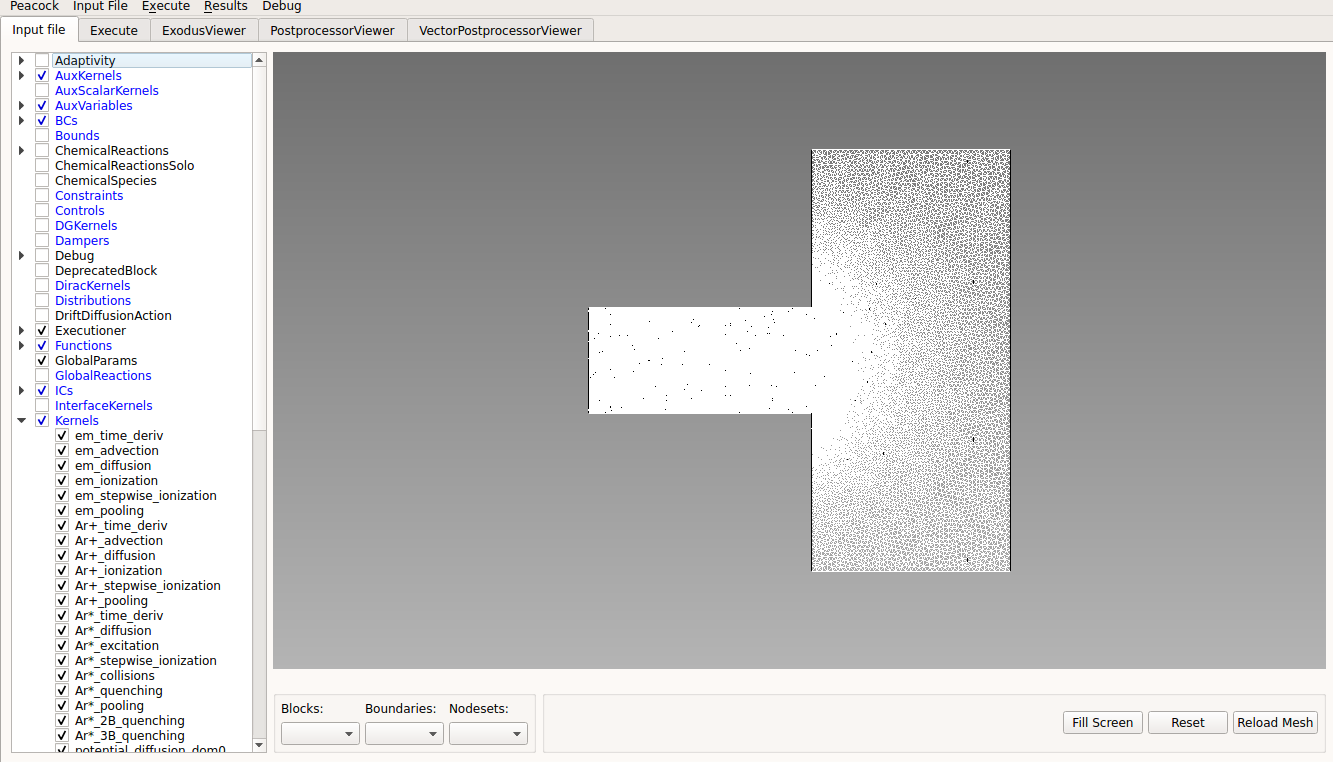
\includegraphics[scale=0.35]{zapdos_content/media/Zapdos_Peacock.png}
  \caption{Example of a Zapdos input file in Peacock}
\end{figure}

\begin{figure}[!h]
  \centering
  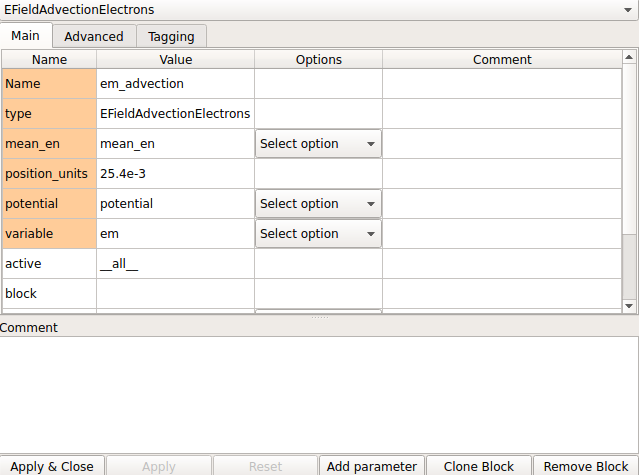
\includegraphics[scale=0.5]{zapdos_content/media/em_advection_peacock.png}
  \caption{Example for a kernel option menu in Peacock}
\end{figure}

  \section{1D: CCP Discharge}
  This tutorial is based on the work by Lymberopoulos \cite{1D_GEC} and the input file can be found as \\
  zapdos/problems/Lymberopoulos\_with\_argon\_metastables.i. This input file simulates a 1Torr parallel plate argon plasma with one electrode powered at 100V 13.56Hz RF and the other electrode grounded. This simulation also includes argon metastables. The contents of the input can be found in Appendix A1.

 \section{2D: GEC Reference Cell}
 This tutorial is based on the work by Lymberopoulos \cite{2D_GEC_100mTorr} and the input file can be found as \\
 zapdos/problems/Lymberopoulos\_with\_argon\_metastables\_2D\_At100mTorr.i.  This input file simulates a 100 mTorr argon plasma within the GEC reference cell. The top and bottom electrodes are powered in such a way that the peak-to-peak voltage is 100V at 13.56Hz and the walls of the chamber is grounded. There is also a thin piece of insulator that acts as a dielectric boundary and this simulation includes argon metastables. The contents of the input can be found in Appendix A2.

 \section{Hands-on Work}
 \subsection{GEC at Higher Pressures}
 In this exercise, the goal is to replicate the discharge parameters found in the work due by Lymberopoulos in \cite{2D_GEC_1Torr}. One may notice this discharge is very similar to the one the 100m Torr case in the previous example, expect that the pressure is 1Torr and the peak-to-peak voltage is 60V. For help with this exercise, the completed input file can be found at zapdos/problems/Lymberopoulos\_with\_argon\_metastables\_2D\_At1Torr.i.

  \subsection{Actions With Zapdos and CRANE}
  Action blocks are a type of block that can call multiple different kernels, BCs, and materials at once. This is helpful when dealing with large sets of equations. There are two main actions in Zapdos/CRANE, DriftDiffusionAction and Reactions. The example code below shows the required inputs for these actions. The goal of this exercise is to rewrite the Lymberopoulos\_with\_argon\_metastables.i input file with these action blocks (this can be done in both a text editor or Peacock). For help with this exercise, the completed input file can be found at \\
  zapdos/problems/RF\_Plasma.i.

  \begin{verbatim}
[DriftDiffusionAction]
  [Plasma]
    electrons = em
    charged_particle = Ar+
    Neutrals = Ar*
    potential = potential
    Is_potential_unique = true
    mean_energy = mean_en
    position_units = ${dom0Scale}
    Additional_Outputs = 'ElectronTemperature Current EField'
  []
[]

[Reactions]
  [Argon]
    species = 'Ar* em Ar+'
    aux_species = 'Ar'
    reaction_coefficient_format = 'rate'
    gas_species = 'Ar'
    electron_energy = 'mean_en'
    electron_density = 'em'
    include_electrons = true
    file_location = 'rate_coefficients'
    potential = 'potential'
    use_log = true
    position_units = ${dom0Scale}
    block = 0
    reactions = 'em + Ar -> em + Ar*        : EEDF [-11.56] (reaction1)
                 em + Ar -> em + em + Ar+   : EEDF [-15.7] (reaction2)
                 em + Ar* -> em + Ar        : EEDF [11.56] (reaction3)
                 em + Ar* -> em + em + Ar+  : EEDF [-4.14] (reaction4)
                 em + Ar* -> em + Ar_r      : 1.2044e11
                 Ar* + Ar* -> Ar+ + Ar + em : 373364000
                 Ar* + Ar -> Ar + Ar        : 1806.6
                 Ar* + Ar + Ar -> Ar_2 + Ar : 39890.9324'
  []
[]
  \end{verbatim}

  \subsection{The Plasma-Liquid Interface}
  A good next step after understanding simulating only plasma is to try to replicate the works by Lindsay in \cite{plasma_water}. This work includes InterfaceKernels and two different domains. In order to uses InterfaceKernels, one must setup interface boundaries with the MeshModifier block. Examples code for the MeshModifer and InterfaceKernels blocks are below. Note: in order to get atmospheric runs working, Zapdos currently needs to used the MoleStabilizing Kernel with a value of 20. For help with this exercise, the completed input file can be found at \\ zapdos/problems/mean$\_$en.i.

  \begin{verbatim}
  [MeshModifiers]
    #Setting the path from plasma to water
    [interface]
        type = SideSetsBetweenSubdomains
        master_block = '0' #plasma
        paired_block = '1' #water
        new_boundary = 'master0_interface'
    []
  []
  \end{verbatim}

  \begin{verbatim}
  [InterfaceKernels]
    #Defining electron advection to the water
    [em_advection]
        type = InterfaceAdvection
        mean_en_neighbor = mean_en
        potential_neighbor = potential
        neighbor_var = em   #electrons in plasma
        variable = emliq    #electrons in water
        boundary = master1_interface
        position_units = ${dom1Scale}
        neighbor_position_units = ${dom0Scale}
    []
    #Defining electron diffusion to the water
    [em_diffusion]
        type = InterfaceLogDiffusionElectrons
        mean_en_neighbor = mean_en
        neighbor_var = em
        variable = emliq
        boundary = master1_interface
        position_units = ${dom1Scale}
        neighbor_position_units = ${dom0Scale}
    []
[]
  \end{verbatim}

  \chapter{Appendix} \label{appendix}
  \section*{A1: Input Code: Lymberopoulos\_with\_argon\_metastables.i}
  \lstinputlisting[basicstyle=\scriptsize]{../tests/Lymberopoulos_rf_discharge/Lymberopoulos_with_argon_metastables.i}
  \section*{A2: Input Code:\\
  Lymberopoulos\_with\_argon\_metastables\_2D\_At100mTorr.i}
  \lstinputlisting[basicstyle=\scriptsize]{../tests/Lymberopoulos_rf_discharge/Lymberopoulos_with_argon_metastables_2D_At100mTorr_CoarseMesh.i}

  %\bibliography{references} % Need to add references.bib file
  %\bibliographystyle{unsrt}

\begin{thebibliography}{9}
\bibitem{Alex_thesis} Lindsay, Alexander David. "Coupling of Plasmas and Liquids." Thesis (Ph.D.)--North Carolina State University, 2016

\bibitem{2D_GEC_100mTorr} Lymberopoulos, Dimitris P. and Economou, Demetre J. "Modeling and simulation of glow discharge plasma reactors." \textit{J. Vac. Sci. Technol. A} \textbf{12} (1994) 1229; https://doi.org/10.1116/1.579300

\bibitem{1D_GEC}Lymberopoulos, Dimitris P. and Economou, Demetre J. "Fluid simulations of glow discharges: Effect of metastable atoms in argon." \textit{J. Appl. Phys.} \textbf{73} (1993) 3668; https://doi.org/10.1063/1.352926

\bibitem{2D_GEC_1Torr} Lymberopoulos, Dimitris P. and Economou, Demetre J. "Fluid simulations of radio frequency glow discharges: Two-dimensional argon discharge including metastables" \textit{Appl. Phys. Lett.} \textbf{63} (1993) 18

\bibitem{plasma_water} Lindsay, Alexander David and \textit{et al.} "Fully coupled simulation of the plasma liquid interface and interfacial coefficient effects" \textit{J. Phys. D: Appl. Phys.} \textbf{49} (2016) 235204

\bibitem{Gmsh} http://gmsh.info/doc/texinfo/gmsh.html

\bibitem{Hagelaar_BC1} Hagelaar G J M, De Hoog F J and Kroesen G M W. "Boundary conditions in fluid models of gas discharges" \textit{Phys. Rev. E} \textbf{62} (2000) 1452–4

\bibitem{Hagelaar_BC2} Sakiyama Y and Graves D B. "Nonthermal atmospheric RF plasma in one-dimensional spherical coordinates: asymmetric sheath structure and the discharge mechanism" \textit{J. Appl. Phys.} \textbf{101} (2007) 073306

\bibitem{AccByAveraging} Ventzek, Peter L. G. and \textit{et al.} "Two-dimensional modeling of high plasma density inductively coupled sources for materials processing" \textit{J. Vac. ScI. Technol. B} \textbf{12} (1994) 461

\bibitem{ShootingMethod} Gogolides, E. and \textit{et al.} "Direct Calculation of Time-Periodic States of Continuum Models of Radio-Frequency Plasma" \textit{Chemical Engineering Science} \textbf{47} (1992) 3839-3855
\end{thebibliography}

\end{document}
